\chapter{Futur}

\section{Ecmascript6}
\label{ch:ecmascript6}

\subsection{Présentation}


JavaScript a parcouru un long chemin depuis ses humbles débuts il y’a à peu prêt vingt ans. Aujourd’hui , les développeurs sont en train d’écrire des milliers de ligne de code qui créent des applications JavaScript complexes. Avant de nous plonger dans les caractéristiques de ES6, vous pouvez regarder le tableau d’ensemble qui est défini dans le projet de spécifications, en termes d'exigences, d’objectifs , de moyen et de thèmes bordés.

L’un des objectifs de ES6 est d’être un meilleur langage pour la création:


\begin{list}{•}{•}
  \item 
  applications complexes
  \item
  bibliothèques
  \item
  générateurs de code
\end{list}

\subsection {Compatibilité}

Le tableau de compatibilité  d’ES6 est très utile, car elle nous indique les caractéristiques pris en charge dans le s navigateurs actuel. Elle nous donne également un lien pratique pour les spécifications de chacun des caractéristiques énumérées.

\begin{center}
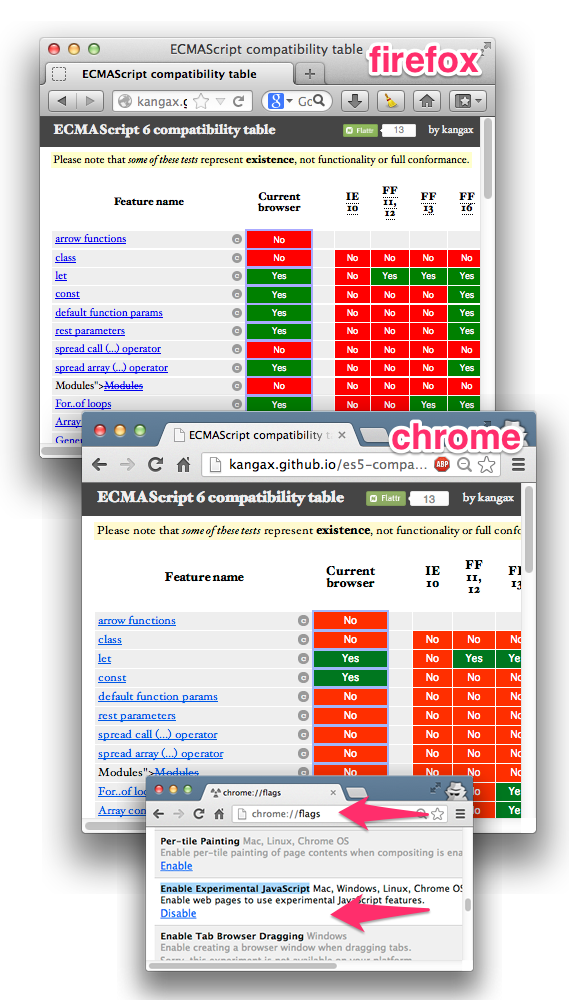
\includegraphics[scale=0.7]{img/es6-compatibility.png}
\label{Plateforme Wakanda}
\end{center}

\subsection{Nouveautés}

Voici ure liste non exhaustive des fonctionnalités qu’apporte EcmaScript 6

\begin{list}{•}{•}
  
  \item 
  Block scoping with let (en utilisant Firefox )
  \item
  Bloc scoping with const (en utilisant Chome )
  \item
  Classes (en utilisant Traceur)
  \item
  Default function parameters (en utilisant TypeScript)
  \item
  Collections (en utilisant NodeJS)
  \item
  Destructuring (en utilisant Firefox)
  \item
  Rest parameters \& Spead operator (en utilisant Grunt plugin Traceur)
  \item
  Iterators (en utilisant Firefox)
  \item
  Array compréhension (en utilisant Firefox)
  \item
  Modules (en utilisant ES6 Module Tranpiler)

\end{list}



